% To je predloga za poročila o domačih nalogah pri predmetih, katerih
% nosilec je Blaž Zupan. Seveda lahko tudi dodaš kakšen nov, zanimiv
% in uporaben element, ki ga v tej predlogi (še) ni. Več o LaTeX-u izveš na
% spletu, na primer na http://tobi.oetiker.ch/lshort/lshort.pdf.
%
% To predlogo lahko spremeniš v PDF dokument s pomočjo programa
% pdflatex, ki je del standardne instalacije LaTeX programov.

\documentclass[a4paper,11pt]{article}
\usepackage{a4wide}
\usepackage{fullpage}
\usepackage[utf8x]{inputenc}
\usepackage[slovene]{babel}
\selectlanguage{slovene}
\usepackage[toc,page]{appendix}
\usepackage[pdftex]{graphicx} % za slike
\usepackage{setspace}
\usepackage{color}
\definecolor{light-gray}{gray}{0.95}
\usepackage{listings} % za vključevanje kode
\usepackage{hyperref}
\usepackage{float}
\usepackage{verbatim}
\renewcommand{\baselinestretch}{1.2} % za boljšo berljivost večji razmak
\renewcommand{\appendixpagename}{Priloge}

\lstset{ % nastavitve za izpis kode, sem lahko tudi kaj dodaš/spremeniš
language=Python,
basicstyle=\footnotesize,
basicstyle=\ttfamily\footnotesize\setstretch{1},
backgroundcolor=\color{light-gray},
}

\title{Sedma domača naloga}
\author{Anže Pečar (63060257)}
\date{\today}

\begin{document}

\maketitle

\section{Uvod}
Cilj doma"ce naloge je bil preizkusiti delovanje logisti"cne regresije z regularizacijo na podatkih za tekmovanje iz podro"cja kemoinfromatike.
\section{Metode}
\subsection{Logisti"cna regresija}
Logisti"cna regresija se uporablja pri binarnih klasifikacijskih problemih. Za te probleme sicer lahko uporabimo tudi linearno regresijo, vendar je, kot smo videli na predavanjih, trivialno sestaviti primer, kjer se linearna regresija ne izka"ze. Intuitivno tudi nima nobenega smisla, da nam hipoteza $h_\Theta(x)$ vra"ca vrednosti manj"sa od 0 in ve"cja od 1, "ce pa vemo, da je $y \in \{0, 1\}$.

V na"so hipotezo vstavimo logisti"cno funkcijo, da dobimo 

\[
	h_\Theta(x) = \frac{1}{1 + e^{-\Theta^Tx}}.
\]


\subsection{Cenovna funkcija}

Cenovna funkcija, ki jo "zelimo "zmanj"sati je tako imenovana \textit{log loss} funkcija. Definirana je na naslednji na"cin
\[
logloss = -\frac{1}{N}\sum_{i=1}^Ny_i\log\left(\hat{x_i}\right)\left(1-y_i\right)\log\left(1-\hat{x_i}\right).
\]
Za vrednost $\hat{x_i}$ smo uporabili logisti"cno funkcijo po naslednji ena"cbi
\[
	\hat{y_i} = h_\Theta(x_i).
\]


\subsection{Gradient}
Da bi maksimizirali verjetje (\textit{liklehood}) $L(\Theta) = p(\vec{y} |X;\Theta)$, lahko uporabimo metodo najhitrej"sega sestopa (\textit{gradient ascent}). V vektorski notaciji ga zapi"semo kot $\Theta = \Theta + \alpha*\Delta_\Theta l(\Theta)$, kjer je $l(\Theta) = log L(\Theta)$. Iz vektorskega zapisa lahko izpeljemo stohasti"cno formulo, ki je zelo podobna tisti, ki smo jo uporabili pri linearni regresiji
\[
	\Theta_j = \Theta_j + \alpha(y^{(i)} - h_\Theta(x^{(i)}))x^{(i)}_j.
\]
Razlika je seveda v tem, da je tukaj $h_\Theta(x^{(i)}))$ logisti"cna funkcija, kot smo jo definirali zgoraj.

\section{Podatki in opis problemske domene}

Podatki so iz tekmovanja iz podro"cja kemoinformatike. Problemska domena ima 1776 atributov in 3751 primerov. Vrednosti atributov so med 0 in 1, kar precej pa jih ima samo dve razli"cni vrednosti.

\section{Rezultati}
Rezultati 5-kratnega pre"cnega preverjanja so zbrani v tabeli \ref{pt}. Kot je razvidno iz tabele smo najbolj"si rezultat dobili pri lambda\_ 0.01. Nismo pa uspeli izbolj"sati rezultata prej"sne doma"ce naloge, kjer smo z RF algoritmom dobili logloss 0.4643. 
\begin{table}[htbp]
\caption{Rezultati}
\label{pt}
\begin{center}
\begin{tabular}{llp{3cm}}
lambda\_ &  log\_loss\\
\hline
0.1 & 0.569092454919\\
0.01 & 0.506691088418\\
0.001 & 0.557776033395\\
0.0001 & 0.745162922321\\
0.0 & 2.86933161772\\

\hline
\end{tabular}
\end{center}
\end{table}


%\begin{figure}[H]
%\begin{center}
%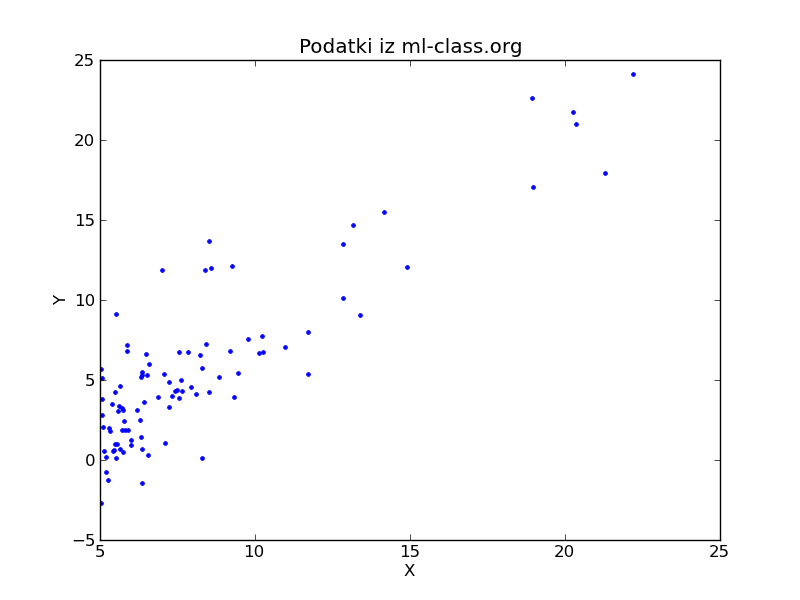
\includegraphics[scale=0.3]{ml-data.png}
%\caption{Podatki iz ml-class.org}
%\end{center}
%\label{mldata}
%\end{figure}


\section{Izjava o izdelavi domače naloge}
Domačo nalogo in pripadajoče programe sem izdelal sam.


\begin{thebibliography}{9}

\bibitem{mining}
   Ian H. Witten \& Eibe Frank,
   \emph{Data Mining Practical Machine Learning Tools and Techniques, Second Edition}
   Morgan Kaufmann Publishers,  
   2005.

\end{thebibliography}

\end{document}
